\chapter[Simulador]{Simulador de ejecución de flujos de trabajo}

En los capítulos anteriores, se han revisado los principales elementos del problema de la planificación de flujos de trabajo en entornos de cómputo distribuido. Se estudió también el concepto de flujo de trabajo y sus propiedades. También se han detallado los enfoques de cómputo distribuido comunes en la planificación de flujos de trabajo. Además, se ha estudiado el problema de planificación elemental y su aplicación al problema específico de flujos de trabajo. De este modo, se puede notar que son varios los factores que se tienen que tomar en cuenta para construir software para flujos de trabajo en entornos de cómputo distribuido.

Con el fin de facilitar el estudio de los algoritmos de planificación de flujos de trabajo y de proveer a la comunidad científica de cloud computing de una plataforma para analizar el desempeño de nuevos algoritmos de planificación con respecto a algoritmos consolidados, se construyó un simulador de ejecución de flujos de trabajo. El simulador está construido con el lenguaje de programación Java. También, se utilizó Maven \cite{maven2014} para administrar el proceso de compilación de código y JUnit \cite{junit2014} para administrar la aplicación de pruebas unitarias. Además, el código está disponible como software libre \cite{dominofire2014workflowsimulator} para su libre utilización en otros proyectos.

Los algoritmos de planificación implementados en el simulador son: Miope (\ref{alg:myopic}, \ref{code:myopic}), MinMin (\ref{alg:min-min}, \ref{lst:xmin_main}) y MaxMin (\ref{alg:max-min}, \ref{lst:xmin_main}). Cabe recordar que el algoritmo Miope es un algoritmo voraz que busca el recurso que pueda ejecutar la tarea lo más pronto posible. Por otro lado, los algoritmos MinMin y MaxMin buscan recursos que puedan minimizar tanto la duración de las tareas listas como el tiempo en el que inician la ejecución de las tareas. Luego, en el caso de MaxMin, se busca la tarea que tarde más tiempo en ejecutarse. En el caso de MinMin, se busca la tarea que tarde menos en ejecutarse.

Para simplificar la construcción del simulador, se asumieron siete suposiciones:

\begin{enumerate}
\item Los recursos pueden ejecutar todas las tareas.
\item Los recursos ejecutan una sola tarea a la vez.
\item Todos los recursos están conectados entre sí.
\item La transferencia de datos entre recursos es instantánea.
\item Una tarea es considerada lista para planificarse si todos sus predecesores inmediatos han sido planificados.
\item La ejecución de las tareas en los recursos no falla.
\item Una tarea es planificada una sola vez.
\end{enumerate}

\section{Clases comunes para los algoritmos}
El diseño de las clases y objetos se hizo de tal modo que los elementos más comunes de los algoritmos fueran representados en una clase. Así, describiremos primero las clases \texttt{Task}, \texttt{Resource} y \texttt{Schedule}, para luego describir la clase \texttt{Workflow} y las clases que implementan los algoritmos: \texttt{Myopic}, \texttt{MinMin} y \texttt{MaxMin}. En la figura \ref{fig:uml_class} se muestra el diagrama de clases que modela los elementos del problema de planificación de flujos de trabajo. Estas clases se encuentran en el paquete \texttt{org.perez.workflow.elements}, las cuales describiremos a continuación.

\begin{figure}
\begin{center}
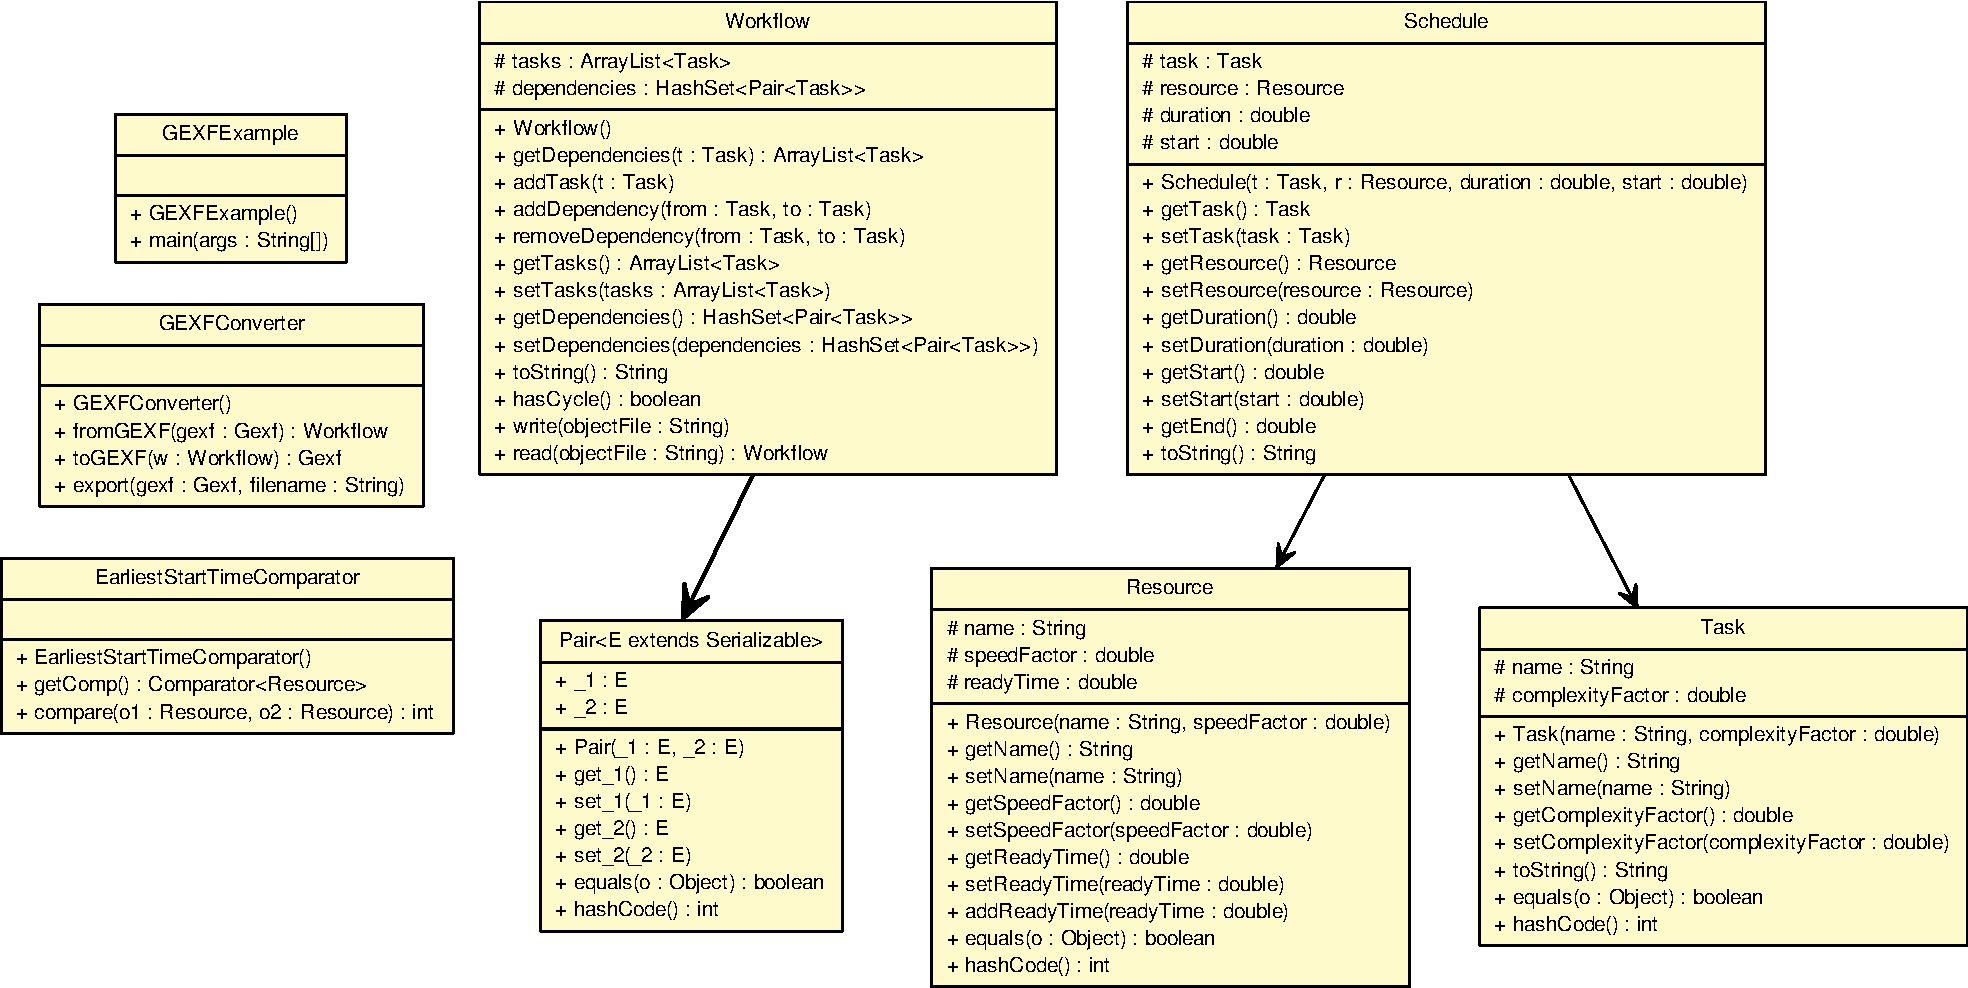
\includegraphics[width=1.2\textwidth,angle=90]{imagenes/elements_uml.pdf}
\end{center}
\label{fig:uml_class}
\caption{Diagrama de clases de los elementos comunes de los algoritmos.}
\end{figure}

\begin{itemize}

\item{\textbf{Clase \texttt{Task}}: Representa una tarea que forma parte de un flujo de trabajo. Cada tarea tiene un nombre que debe ser único en el flujo de trabajo del que forma parte. También, la tarea contiene un factor de complejidad, que es un número que representa qué tan complicado es ejecutar esta tarea. La idea básica es que a mayor factor de complejidad, mayor es el tiempo requerido para ejecutar la tarea o un recurso más rápido es necesario para ejecutar la tarea de forma eficiente. Junto con el factor de velocidad de un recurso (que se verá en la descripción de la clase \texttt{Resource}), el tiempo de ejecución de una tarea en un recurso particular se calcula con la siguiente fórmula:
\begin{equation}
  \text{Tiempo de ejecución} = \frac{\text{Factor de complejidad}}{\text{Factor de velocidad}}
\end{equation}}

\item \textbf{Clase \texttt{Resource}}: En esta clase se representa a un recurso que puede ejecutar tareas de un flujo de trabajo. De forma similar a la clase \texttt{Task}, un recurso tiene un nombre --que no es necesario que sea único-- y un factor de velocidad que indica la rapidez con la que dicho recurso puede ejecutar una tarea.

\item \textbf{Clase \texttt{Schedule}}: Representa una planificación de una tarea en un recurso. Cada objeto de esta clase guarda la tarea y el recurso que fueron asignados, el tiempo en que se empezará a ejecutar la tarea y el tiempo estimado de ejecución de la tarea en el recurso.

\item \textbf{Clase \texttt{Workflow}}: La clase \texttt{Workflow} representa un flujo de trabajo, compuesto de tareas y las relaciones de precedencia entre tareas. Cabe aclarar que no se permite que existan tareas con el mismo nombre y también se verifica que las relaciones de precedencia entre las tareas formen un grafo dirigido acíclico.

\item \textbf{Clases Adicionales}: La clase \texttt{Pair} es una tupla de dos valores, la cual es utilizada ampliamente en los algoritmos de planificación. La clase \texttt{GEXFConverter} contiene métodos para guardar los flujos de trabajo en archivos con formato GEXF \cite{gexf2014}, el cual es utilizado en software como Gephi \cite{bastian2009gephi} para visualizar grafos. La clase \texttt{EarliestStartTimeComparator} implementa un comparador que es utilizado en el algoritmo Miope para mantener una lista de recursos ordenada por el tiempo de disponibilidad más corto.
\end{itemize}

\section{Código de los algoritmos de planificación}
En esta sección, detallaremos las decisiones de diseño que fueron necesarias para implementar los algoritmos. Como se verá en cada uno de los algoritmos, todos tienen detalles específicos que salen a la luz a la hora de programar. Cada algoritmo está codificado en una clase y cada una de estas clases contiene un método estático de la forma:

\begin{center}
\begin{lstlisting}[numbers=none]
List<Schedule> schedule(Workflow w, List<Resource> resourceList) { ... }
\end{lstlisting}
\end{center}

En la figura \ref{fig:uml_class_scheduler} están las clases que implementan los algoritmos de planificación. También en esta figura están representadas las clases auxiliares utilizadas tanto en los algoritmos y en las pruebas. La clase \texttt{Utils} tiene métodos para verificar si una planificación es correcta. También contiene métodos para imprimir las planificaciones, útil para las sesiones de depuración. Otro método importante a mencionar es \texttt{createRGanttScript()}, el cual genera un script en el lenguaje de programación estadística R \cite{Rlang2014} para graficar la planificación de un flujo de trabajo.

\begin{figure}
\begin{center}
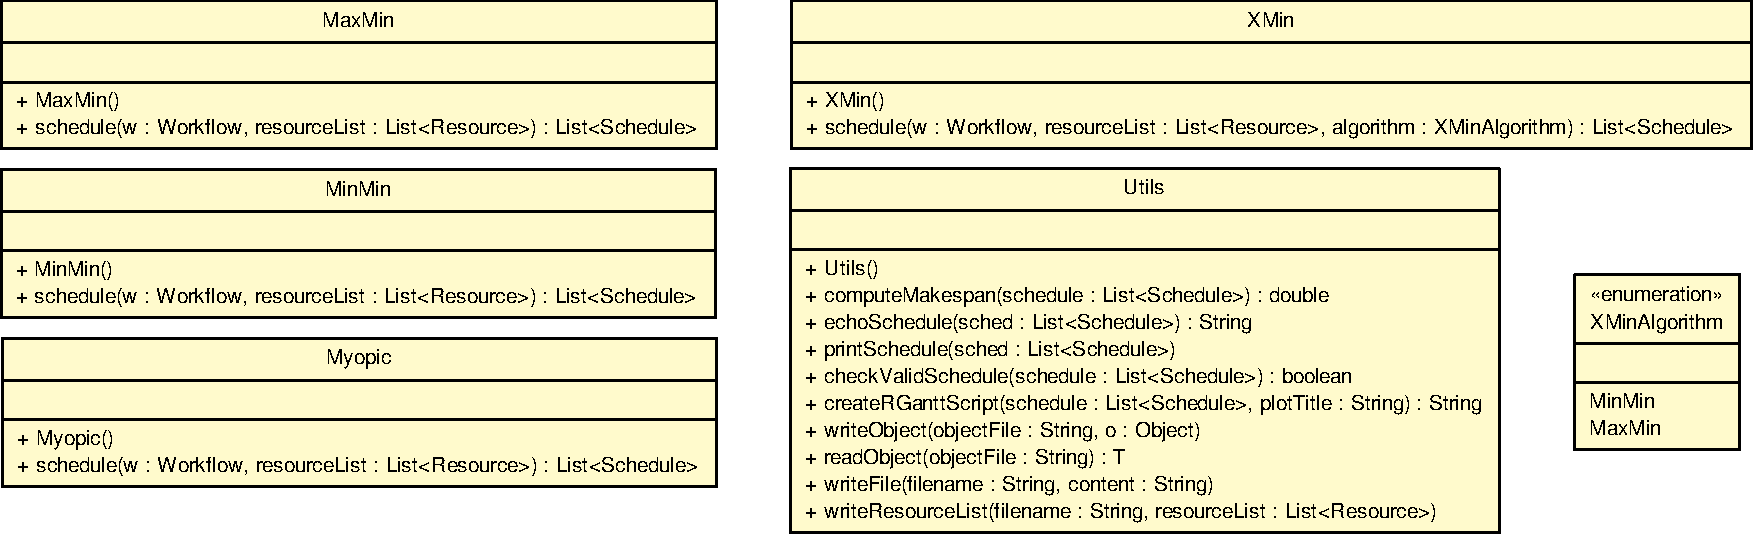
\includegraphics[width=1.2\textwidth, angle=90]{imagenes/scheduler_uml.pdf}
\end{center}
\label{fig:uml_class_scheduler}
\caption{Diagrama de clases de los algoritmos y clases auxliares.}
\end{figure}

A continuación, se describirán los detalles de implementación de cada uno de los algoritmos de planificación.

\subsection{Algoritmo Miope}
Como se vio en el capítulo \ref{chap:scheduling_algorithms}, el algoritmo Miope asigna tareas a recursos de tal modo que se empiecen a ejecutar lo más pronto posible. Aunque la idea básica resulte fácil de entender, hay algunas cuestiones que deben ser resueltas para implementar este algoritmo. En el código \ref{code:myopic} se encuentra el código del algoritmo Miope, el cual utiliza las clases de los elementos comunes antes descritos. 

Primero, hay que hacer una distinción entre \emph{tareas planificadas} y \emph{tareas listas}. Una tarea está planificada si ya está asignada a uno y sólo un recurso. Cabe aclarar que en el simulador no se permite que una tarea sea asignada a varios recursos. Ahora bien, una tarea está lista para planificar si sus predecesores inmediatos o padres han sido planificados. Esto asegura que se respeten las dependencias entre las tareas a la hora de planificar.

También, hay que tomar en cuenta cómo obtener tareas que estén listas para planificar. En el caso del algoritmo Miope, se evalúa exhaustivamente la lista de tareas disponibles \texttt{readyTasks} (línea \ref{code:myopic_readyTasks} del código \ref{code:myopic}) en busca de una tarea lista para planificar. La llamada al método \texttt{Utils.checkParents(task, schedTasks, workflow)} (línea \ref{code:myopic_checkParents} del código \ref{code:myopic}) devuelve \texttt{true} si la tarea \texttt{task} es una \emph{tarea lista} para planificar. Este método (código \ref{code:utils_checkParents}) determina si todos los padres de una tarea dada se encuentran en la lista de tareas planificadas.

\begin{lstlisting}[language=java,label={code:utils_checkParents},caption={Método que verifica si los padres de una tarea están planificados.},float]
boolean checkParents(Task t, ArrayList<Task> sched, Workflow w) {
  //TODO: do we need check parents recursively?
  ArrayList<Task> parents = w.getDependencies(t);
  for(Task parentTask: parents)
    if(!sched.contains(parentTask))
      return false;
  return true;
}
\end{lstlisting}

Una vez que se obtiene la tarea lista para planificar, se busca el recurso al que se le asignará la tarea. Así, se mantiene una cola de prioridad \texttt{R} (línea \ref{code:myopic_R} del código \ref{code:myopic}) de los recursos con el tiempo de disponibilidad más pronto. Como esta cola de prioridad es un montículo, sólo necesitamos consultar la raíz del montículo para saber cuál es el recurso con el menor tiempo de disponibilidad.

Con el recurso seleccionado de la cola de prioridad, se hacen los cálculos (líneas \ref{code:myopic_scIni}-\ref{code:myopic_scEnd} del código \ref{code:myopic}) del tiempo de ejecución y el tiempo de inicio de la tarea en el recurso elegido. Para el caso del tiempo de inicio, en la línea \ref{code:myopic_scPRT} del código \ref{code:myopic} se hace una llamada al método \texttt{Utils.parentsReadyTime(task, scheduleList, workflow)}, el cual obtiene el instante de tiempo más pronto en el que todos los padres de una tarea han sido ejecutados. Este método, mostrado en el código \ref{code:utils_parentsReadyTime}, busca en la lista de tareas planificadas si se encuentran los padres de la tarea dada y mantiene un registro del tiempo que tardan en ejecutarse estos padres.

\begin{lstlisting}[language=java,label={code:utils_parentsReadyTime},caption={Método que calcula el tiempo mínimo en el que los padres de una tarea dada han sido ejecutados.},float]
double parentsReadyTime(Task t, List<Schedule> partialSchedule, Workflow w) {
  double parentsReadyTime = 0;
  ArrayList<Task> parents = w.getDependencies(t);
  //asumimos que tenemos tareas unicas y planificaciones unicas
  for(Task parentTask: parents)
    for(Schedule s: partialSchedule)
      if(parentTask.equals(s.getTask()))
        parentsReadyTime = Math.max(parentsReadyTime, s.getStart() + s.getDuration());

  return parentsReadyTime;
}
\end{lstlisting}

Estos cálculos son utilizados para crear un objeto del tipo \texttt{Schedule} que representa la planificación de la tarea en el recurso. Más adelante, se vuelve a crear la cola de prioridad (línea \ref{code:myopic_updateR} del código \ref{code:myopic}) para conocer en la siguiente iteración del algoritmo cuál es el recurso con el menor tiempo de disponibilidad. Por último, el algoritmo termina cuando ya no hay más tareas listas para planificar (i.e. cuando la lista \texttt{readyTasks} esté vacía).

\begin{lstlisting}[language=java,label={code:myopic},caption={Algoritmo Miope},float]
List<Schedule> schedule(Workflow w, List<Resource> resourceList) {
  Utils.checkScheduleParams(w, resourceList);
  //lista de tareas no planificadas
  ArrayList<Task> schedTasks = new ArrayList<Task>();
  ArrayList<Task> allTasks = new ArrayList<Task>(w.getTasks());
  ArrayList<Task> readyTasks = null; (*@\label{code:myopic_readyTasks}@*)
  ArrayList<Schedule> scheduleList = new ArrayList<Schedule>();
  //necesito un heap para mantener a los recursos mas pronto disponibles
  PriorityQueue<Resource> R = new PriorityQueue<Resource>(resourceList.size(), EarliestStartTimeComparator.getComp()); (*@\label{code:myopic_R}@*)
  R.addAll(resourceList);
  Task t; Resource r;
  while(!allTasks.isEmpty()) {
    //puedes sacar subconjuntos de todas las tareas
    readyTasks = new ArrayList<Task>();
    for(Task tt: allTasks)
      if(!schedTasks.contains(tt) && Utils.checkParents(tt, schedTasks, w)) (*@\label{code:myopic_checkParents}@*)
        readyTasks.add(tt);
    Iterator<Task> it = readyTasks.iterator();
    while(it.hasNext()) {
      t = it.next(); r = R.peek(); (*@\label{code:myopic_scIni}@*)
      double d = t.getComplexityFactor() / r.getSpeedFactor();
      double st = Math.max(r.getReadyTime(), Utils.parentsReadyTime(t, scheduleList, w)); (*@\label{code:myopic_scPRT}@*)
      Schedule s = new Schedule(t, r, d, st); (*@\label{code:myopic_scEnd}@*)
      allTasks.remove(t);
      schedTasks.add(t);
      r.setReadyTime(st);
      r.addReadyTime(d);
      //Update resource priority queue
      R = new PriorityQueue<Resource>(resourceList.size(), EarliestStartTimeComparator.getComp()); (*@\label{code:myopic_updateR}@*)
      R.addAll(resourceList);
      scheduleList.add(s);
    }
  }
  return scheduleList;
}
\end{lstlisting}

\subsection{Algoritmo MaxMin y MinMin}
Para los algoritmos MaxMin y MinMin se reutilizaron los métodos estáticos de la clase \texttt{Utils}: \texttt{parentsReadyTime()} y \texttt{checkParents()}, que fueron utilizados en el algoritmo Miope. Como se indica en la sección \ref{alg:def_maxmin} del apéndice, hay algunas definiciones que son comunes para ambos algoritmos. Estas definiciones están expresadas en el código \ref{code:xmin_defs}.

\begin{lstlisting}[language=java,label={code:xmin_defs},caption={Definiciones comunes para MaxMin y MinMin.},float]
import static java.lang.Math.max; 
import static org.perez.workflow.scheduler.Utils.parentsReadyTime;

// ...

/** Estimated Availability Time */
double EAT(Task t, Resource r) { return r.getReadyTime(); }

/** Estimated Execution Time */
double EET(Task t, Resource r) { 
  return t.getComplexityFactor() / r.getSpeedFactor(); 
}

/** File Available Time */
double FAT(Task t, Resource r, Workflow w, List<Schedule> partialSchedule) {
  //tomamos el tiempo de los padres como el tiempo de archivos listo
  return max(r.getReadyTime(), parentsReadyTime(t, partialSchedule, w));
}

/** Estimated Completion Time */
double ECT(Task t, Resource r, Workflow w, List<Schedule> partialSchedule) {
  return EET(t, r) + max(EAT(t,r), FAT(t,r, w, partialSchedule));
}
\end{lstlisting}

Como los algoritmos MaxMin y MinMin son muy similares, se hizo un sólo método que encapsula el código en común entre ambos algoritmos. Este método se encuentra en el código \ref{lst:xmin_main}. Además, con el parámetro \texttt{alg}, se puede elegir si se ejecuta el algoritmo MaxMin o el algoritmo MinMin. Este método prepara la lista de tareas listas (líneas \ref{lst:xmin_main_readyIni}-\ref{lst:xmin_main_readyEnd}), luego obtiene las planificaciones de las tareas listas (línea \ref{lst:xmin_main_sched}). Después, actualiza la lista de tareas planificadas (\texttt{schedTasks}) y la lista global \texttt{allTasks}. Nuevamente, el algoritmo termina cuando la lista global está vacía.

\begin{lstlisting}[language=java,label={lst:xmin_main},caption={Método principal para los algoritmos MaxMin y MinMin.},float]
List<Schedule> schedule(Workflow w, List<Resource> resourceList, XMinAlgorithm alg) {
  Utils.checkScheduleParams(w, resourceList); //validacion de argumentos

  ArrayList<Task> schedTasks = new ArrayList<Task>();
  ArrayList<Task> allTasks = new ArrayList<Task>(w.getTasks());
  ArrayList<Task> readyTasks = null;
  List<Schedule> scheduleList = new ArrayList<Schedule>();
  while(!allTasks.isEmpty()) {
    //prepara el conjunto de tareas lista a planificar
    readyTasks = new ArrayList<Task>(); (*@\label{lst:xmin_main_readyIni}@*)
    for(Task t: allTasks)
      if(!schedTasks.contains(t) && Utils.checkParents(t, schedTasks, w))
        readyTasks.add(t); (*@\label{lst:xmin_main_readyEnd}@*)
    //obtiene la planificacion de tareas listas
    scheduleList = scheduleXMin(w, resourceList, readyTasks, scheduleList, alg); (*@\label{lst:xmin_main_sched}@*)
    for(Schedule s: scheduleList) { //actualiza allTasks y schedTasks
      Task t = s.getTask();
      if(!schedTasks.contains(t))
        schedTasks.add(t);
      if(allTasks.contains(t))
        allTasks.remove(t);
    }
  }

  return scheduleList;
}
\end{lstlisting}

Luego, en los códigos \ref{code:xmin_detail_1}, \ref{code:xmin_detail_2} y \ref{code:xmin_detail_3} se encuentra método \texttt{scheduleXMin()} que planifica las tareas listas. En el primer código (\ref{code:xmin_detail_1}) se puede notar los ciclos \texttt{for} que calculan el tiempo estimado de terminación --$ECT(t,r)$-- para cada tarea lista y para cada recurso (líneas \ref{code:xmin_detail_1_forIni}-\ref{code:xmin_detail_1_forEnd}), manteniendo aquel recurso $r$ que minimice $ECT(t,r)$ para cada tarea $t$ (líneas \ref{code:xmin_detail_1_minECTini}-\ref{code:xmin_detail_1_minECTend} y \ref{code:xmin_detail_1_minECTval}-\ref{code:xmin_detail_1_minECTidx}).

\begin{lstlisting}[language=java,label={code:xmin_detail_1},caption={Método de MaxMin/MinMin que planifica las tareas (parte 1)},float]
List<Schedule> scheduleXMin(Workflow w, List<Resource> resourceList, 
  List<Task> availTasks, List<Schedule> partialSched, XMinAlgorithm algorithm) {
  int n_tasks = availTasks.size(),n_resources = resourceList.size();
  double ECT[][] = new double[n_tasks][n_resources];
  double MCT[] = new double[n_tasks];
  int min_mct_r_idx = -1, x_t_idx = -1; double min_mct, x_mct;
  while(!availTasks.isEmpty()) {
    int R_t_idx[] = new int[availTasks.size()];
    for(int i_t=0; i_t<availTasks.size(); i_t++) { (*@\label{code:xmin_detail_1_forIni}@*)
      Task t = availTasks.get(i_t); //recursos ejecutan cualquier tarea
      min_mct_r_idx = -1; min_mct = Double.MAX_VALUE;
      for(int i_r=0; i_r<resourceList.size(); i_r++) {
        Resource r = resourceList.get(i_r);
        ECT[i_t][i_r] = ECT(t, r, w, partialSched);
        if(ECT[i_t][i_r] < min_mct) { (*@\label{code:xmin_detail_1_minECTini}@*)
          min_mct = ECT[i_t][i_r];
          min_mct_r_idx = i_r;
        } (*@\label{code:xmin_detail_1_minECTend}@*)
      } (*@\label{code:xmin_detail_1_forEnd}@*)
      MCT[i_t] = min_mct; (*@\label{code:xmin_detail_1_minECTval}@*)
      R_t_idx[i_t] = min_mct_r_idx; (*@\label{code:xmin_detail_1_minECTidx}@*)
    }
    //continua en el siguiente codigo...
\end{lstlisting}

En el código \ref{code:xmin_detail_2} se encuentra la sentencia \texttt{switch} que decide si se ejecuta el código que es correspondiente al algoritmo MaxMin o al algoritmo MinMin. Como se ha mencionado anteriormente, el algoritmo MaxMin busca aquella tarea $t$ que tenga el máximo $ECT(t,r_{min}(t))$ ejecutada en el recurso $r_{min}(t)$ que minimice el tiempo de ejecución de la tarea $t$ (líneas \ref{code:xmin_detail_2_maxminIni}-\ref{code:xmin_detail_2_maxminEnd}). Por otro lado, el algoritmo MinMin busca aquella tarea $t$ que tenga el mínimo $ECT(t,r_{min}(t))$ (líneas \ref{code:xmin_detail_2_minminIni}-\ref{code:xmin_detail_2_minminEnd}).

\begin{lstlisting}[language=java,label={code:xmin_detail_2},caption={Método de MaxMin/MinMin que planifica las tareas (parte 2)},float]
    //...continuacion
    switch(algorithm) {
      case MaxMin: //Max-Min: maximizar ECT(t, r) sobre tareas
        x_t_idx = -1; x_mct = Double.MIN_VALUE; (*@\label{code:xmin_detail_2_maxminIni}@*)
        for(int i_t=0; i_t<availTasks.size(); i_t++) {
          if(ECT[i_t][R_t_idx[i_t]] > x_mct) {
            x_mct = ECT[i_t][R_t_idx[i_t]];
            x_t_idx = i_t;
          }
        } (*@\label{code:xmin_detail_2_maxminEnd}@*)
      break;
      case MinMin: //Min-Min: minimizar ECT (t, r) sobre tareas
        x_t_idx = -1; x_mct = Double.MAX_VALUE; (*@\label{code:xmin_detail_2_minminIni}@*)
        for(int i_t=0; i_t<availTasks.size(); i_t++) {
          if(ECT[i_t][R_t_idx[i_t]] < x_mct) {
            x_mct = ECT[i_t][R_t_idx[i_t]];
            x_t_idx = i_t;
          }
        } (*@\label{code:xmin_detail_2_minminEnd}@*)
      break;
    }
    //continua en el siguiente codigo...
\end{lstlisting}

Por último, en el código \ref{code:xmin_detail_3} se calculan el tiempo de inicio y la duración de la tarea en el recurso elegido en el código \ref{code:xmin_detail_2}. También, se actualizan la lista de planificaciones (\texttt{partialSched}, línea \ref{code:xmin_detail_3_partialSched}) y la lista de tareas a planificar (\texttt{availTasks}, línea \ref{code:xmin_detail_3_availTasks}).

\begin{lstlisting}[language=java,label={code:xmin_detail_3},caption={Método de MaxMin/MinMin que planifica las tareas (parte 3)},float]
    //...continuacion
    //Schedule T on R_T
    Task t = availTasks.get(x_t_idx);
    Resource r = resourceList.get( R_t_idx[x_t_idx] );
    double duration =  t.getComplexityFactor() / r.getSpeedFactor();
    double startTime = Math.max(r.getReadyTime(), Utils.parentsReadyTime(t, partialSched, w));
    Schedule s = new Schedule(t,r , duration, startTime);
    partialSched.add(s); (*@\label{code:xmin_detail_3_partialSched}@*)
    //remote T from availTasks
    availTasks.remove(t); (*@\label{code:xmin_detail_3_availTasks}@*)
    //update EAT(R_t)
    r.setReadyTime( startTime );
    r.addReadyTime( duration );
  } //del while de la parte 1

  return partialSched;
}
\end{lstlisting}
